% !TEX root = roll_your_own.tex
\chapter{Aristotlean syllogisms}
\label{chap:Aristotle}

Roy Dyckhoff was an enormous influence on Jape. His program MacLogic \citep{dyckhoff1989malt} showed Bernard and me that a novice could be guided through a formal proof (and we were such novices); after a proof was complete it showed a box-and-line rendering; and it included a Prolog encoding of his intuitionistic decision procedure \citep{dyckhoff1992contraction} which would tell the user when they'd made a false step and further progress was impossible. We were sure we could do better; in particular we designed Jape so that it didn't guide a novice but instead showed them where they were in a proof. But we never managed to incorporate a decision procedure into Jape, and Roy, though he listened politely while we enthusiastically promulgated the advantages of Jape, never let on that it was really that decision procedure which was the point of MacLogic. 

Roy's death in 2018 came as a shock. Just after his death an article of his on Aristotlean syllogisms was published \citep{dyckhoff2019indefinite}. I thought it might be fun to be able to check his proofs in Jape (he'd left them as a `logical exercise'). That paper was partly rooted in the work of von Plato \citep{von2016aristotle}, who showed how Aristotle was using a deductive logic, so I had to deal with that as well.

It was more difficult than I had expected, but I was working on it during the spring 2019 Covid lockdown, so I had time. The results are in \textj{Syllogisms (von Plato).jt}, \textj{Syllogisms (Roy Dyckhoff).jt}, and the files they reference in the \textj{examples/Aristotle} folder.

Von Plato's notation uses four kinds of formula, with terms $P$ and $M$
\begin{quote}
\begin{tabular}{ll}
$∏⁺(P,M)$ & All $P$ are $M$ \\
$∏⁻(P,M)$ & No $P$ is $M$ \\
$∑⁺(P,M)$ & Some $P$ are $M$ \\
$∑⁻(P,M)$ & Some $P$ is not $M$ \\
\end{tabular}
\end{quote}
\begin{figure}[b]
\centering
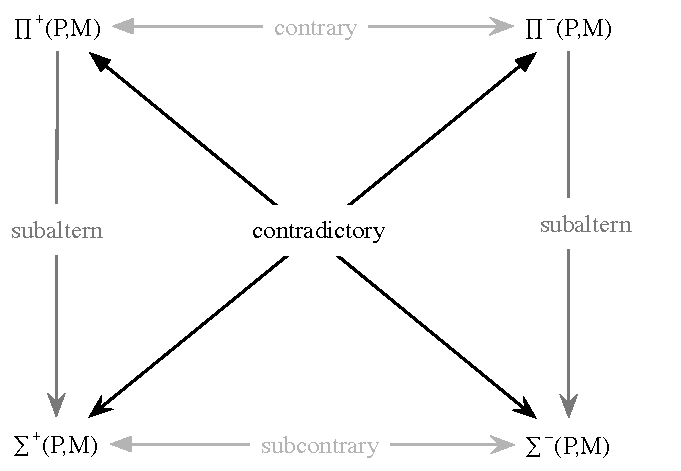
\includegraphics[scale=0.5]{pics/Aristotle/square_of_opposition}
\caption{The square of opposition}
\label{fig:Aristotle:square_of_opposition}
\end{figure}
Figure \ref{fig:Aristotle:square_of_opposition} shows the relationships which mediaeval European logicians drew between these formulas: \emph{contradictory} if one must be false when the other is true; \emph{contrary} if they can't both be true (though they can both be false); \emph{subaltern} if one implies the other. Von Plato makes use of subaltern and contradictory, using superscript tack $^{⊥}$ as a `contradictory' operator; I couldn't find a way to do that in Unicode, so like Dyckhoff I use $^{*}$. $∏⁺(P,M)^{*}$ is $∑⁻(P,M)$; $∏⁻(P,M)^{*}$ is $∑⁺(P,M)$; and in each case the other way around as well. Dyckhoff points out that $A^{{*}{*}}$ is $A$. There is also a notion of `equivalence' or `reversal': $∏⁻(P,M)$ is equivalent to $∏⁻(M,P)$; $∑⁺(P,M)$ to $∑⁺(M,P)$.

Defining the syntax is almost trivial
\begin{japeish}
CLASS VARIABLE P S M X Y               /* TERM, really */\\
CLASS FORMULA A B C\\
\\
PREFIX 100 ∏⁺ ∏⁻ ∑⁺ ∑⁻\\
POSTFIX 50 *\\

SEQUENT IS BAG ⊢ FORMULA
\end{japeish}
%Rules begin fairly normally, except that capriciously I have called tne identity rule `see' (more on this later)
%\begin{japeish}
%INITIALISE seektipselection false       /* yes, we are going to use CUTIN */
%
%RULE see(A) IS INFER A ⊢ A
%
%RULE cut(B) IS FROM B AND B ⊢ C INFER C
%
%STRUCTURERULE IDENTITY   see
%STRUCTURERULE CUT        cut
%
%TACTIC Fail (x) IS SEQ (ALERT x) STOP
%\end{japeish}
The main difficulty of encoding von Plato's logic is the peculiar form of proofs, illustrated in figure \ref{fig:Aristotle:Darapti_various}. Figure \ref{fig:Aristotle:Darapti_1} shows how Jape would display a proof of a particular syllogism (Darapti) in box style with cuts and identity steps hidden. 
\begin{figure}
\centering
\subfigure[with hidden cut and identity]{\centering
\makebox[140pt]{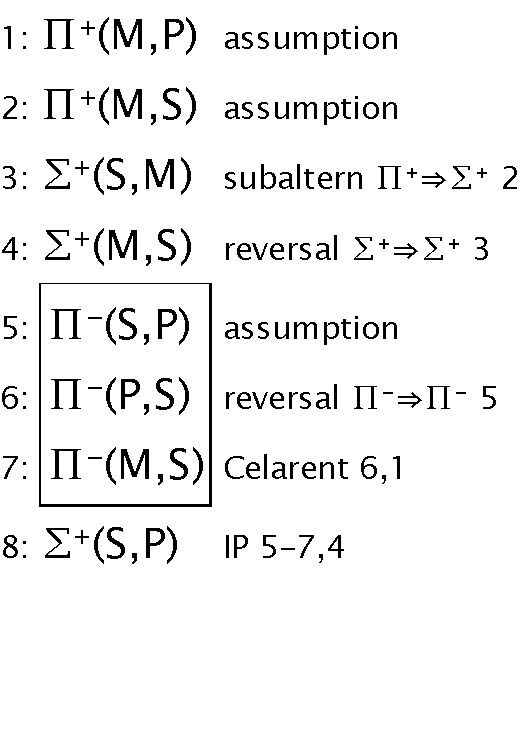
\includegraphics[scale=0.5]{pics/Aristotle/Darapti_1}}\label{fig:Aristotle:Darapti_1}}
\subfigure[with decorated assumption and explicit antecedents]{\centering
\makebox[160pt]{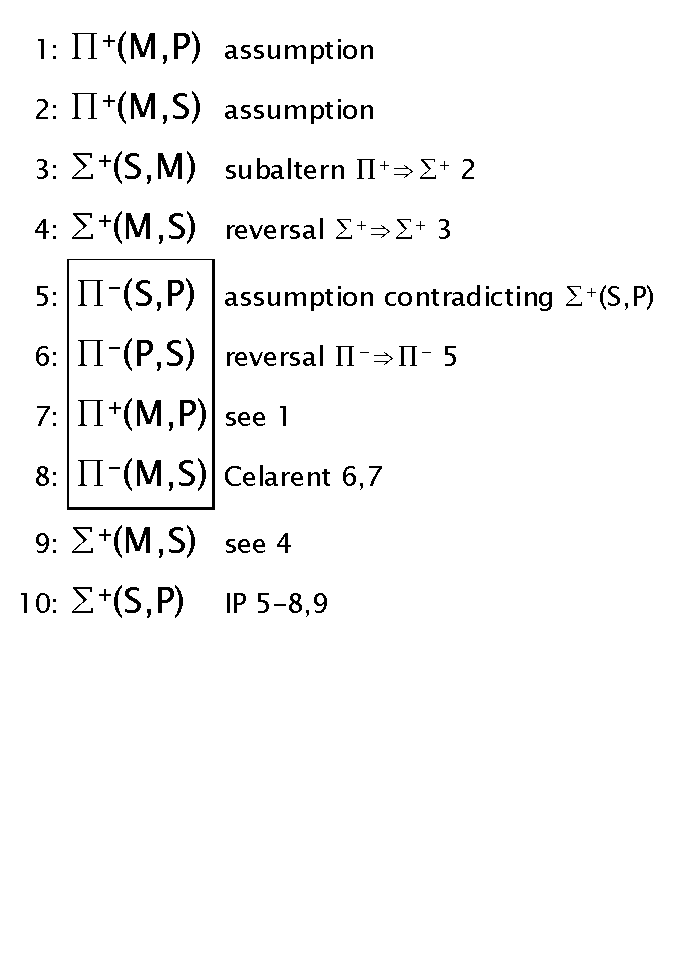
\includegraphics[scale=0.5]{pics/Aristotle/Darapti_2}}\label{fig:Aristotle:Darapti_2}}
\subfigure[without boxes and step names]{\centering
\makebox[155pt]{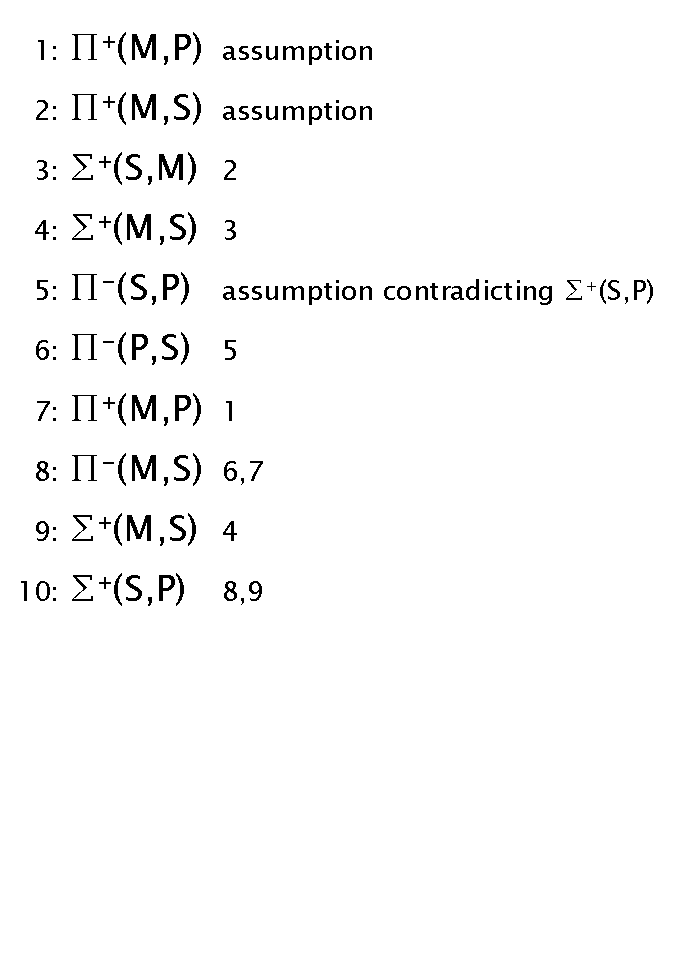
\includegraphics[scale=0.5]{pics/Aristotle/Darapti_3}}\label{fig:Aristotle:Darapti_3}}
\caption{Displaying proofs \`a la von Plato}
\label{fig:Aristotle:Darapti_various}
\end{figure}
Aristotlean linear proofs, according to von Plato, list the antecedent formulae, in order, just before each conclusion step. This can require identity (\textj{see}) lines even though \textj{hidehyp} is true; the first antecedent can be the last line of a box. In addition, the assumption introduced by the \emph{indirect proof} rule IP has to be specially labelled, as is line 5 in figure \ref{fig:Aristotle:Darapti_2}. Finally, the display should be linear without boxes and even without step names, as in figure \ref{fig:Aristotle:Darapti_3}.

The encoding has to make use of new environment variables \textj{priorAntes} (set true), \textj{innerboxes} (set false) and \textj{hidewhy} (set true) to produce these effects, plus a special \textj{LAYOUT} mechanism described below. In addition, the tactics used to apply rules make heavy use of \textj{CUTIN} and \textj{see} to ensure that antecedents are, as far as possible, closed with an identity step -- helpful to the \textj{priorAntes} mechanism. There are radio buttons in the Edit menu to control these variables.

There is a condition on the IP rule which required a new proviso. Essentially the rule is
\begin{japeish}
FROM A* ⊢ B AND B* INFER A
\end{japeish}
-- if the contrary of $A$ proves $B$ and we can separately prove the contrary of $B$, then by \emph{reductio ad absurdum} we can infer $A$. But the assumption $A^{*}$ has to be relevant to the proof: we can't trivially discharge it (i.e. $B$ cannot be $A^{*}$) and we can't have a proof of $B$ which doesn't discharge $A^{*}$ at all. Von Plato says that $A^{*}$ should have a single discharge: from reading his paper and Dyckhoff's I \emph{think} he means that it is discharged only in the left antecedent arm.\footnote{Because his linear proofs have no means of indicating the scope of an assumption, some confusion is to be expected.} The proviso is currently called \textjNTDISCHARGE} (for Non-Trivial discharge), and to avoid too many contrary markers in the proof I made an \textj{ALT} of different versions of \textj{IP}.
\begin{japeish}
RULES IP(B) ARE \\
\tab\tab WHERE NTDISCHARGE ∏⁺(S,P) FROM ∏⁺(S,P) ⊢ B AND B* INFER ∑⁻(S,P) \\ 
 AND WHERE NTDISCHARGE ∏⁻(S,P) FROM ∏⁻(S,P) ⊢ B AND B* INFER ∑⁺(S,P)  \\
 AND WHERE NTDISCHARGE ∑⁺(S,P) FROM ∑⁺(S,P) ⊢ B AND B* INFER ∏⁻(S,P)  \\
 AND WHERE NTDISCHARGE ∑⁻(S,P) FROM ∑⁻(S,P) ⊢ B AND B* INFER ∏⁺(S,P) \\
END
\end{japeish}
\textj{IP} is applied via a tactic in the Rules menu
\begin{japeish}
WHEN (LETGOAL \_A (LAYOUT "IP" ALL IP (LAYOUT ASSUMPTION ("contradicting \%t",\_A)))) \\
\tab\tab\tab                  (ALERT "Please select a consequent to be proved by IP") \\
\end{japeish}
The rule which is applied is either \textj{IP'0}, \textj{IP'1}, \textj{IP'2} or \textj{IP'3}, depending on the conclusion of the step, but the first \textj{LAYOUT} names the step \textj{IP}. The second step applies \textj{LAYOUT} to the first antedecent, giving the text to be appended to `assumption'.

But there's still a problem. The contrary marker $^{*}$ isn't really part of the logic, but it appears in proofs when you use the IP rule. Here, for example, is the first step in the proof of Darapti:
\begin{quote}
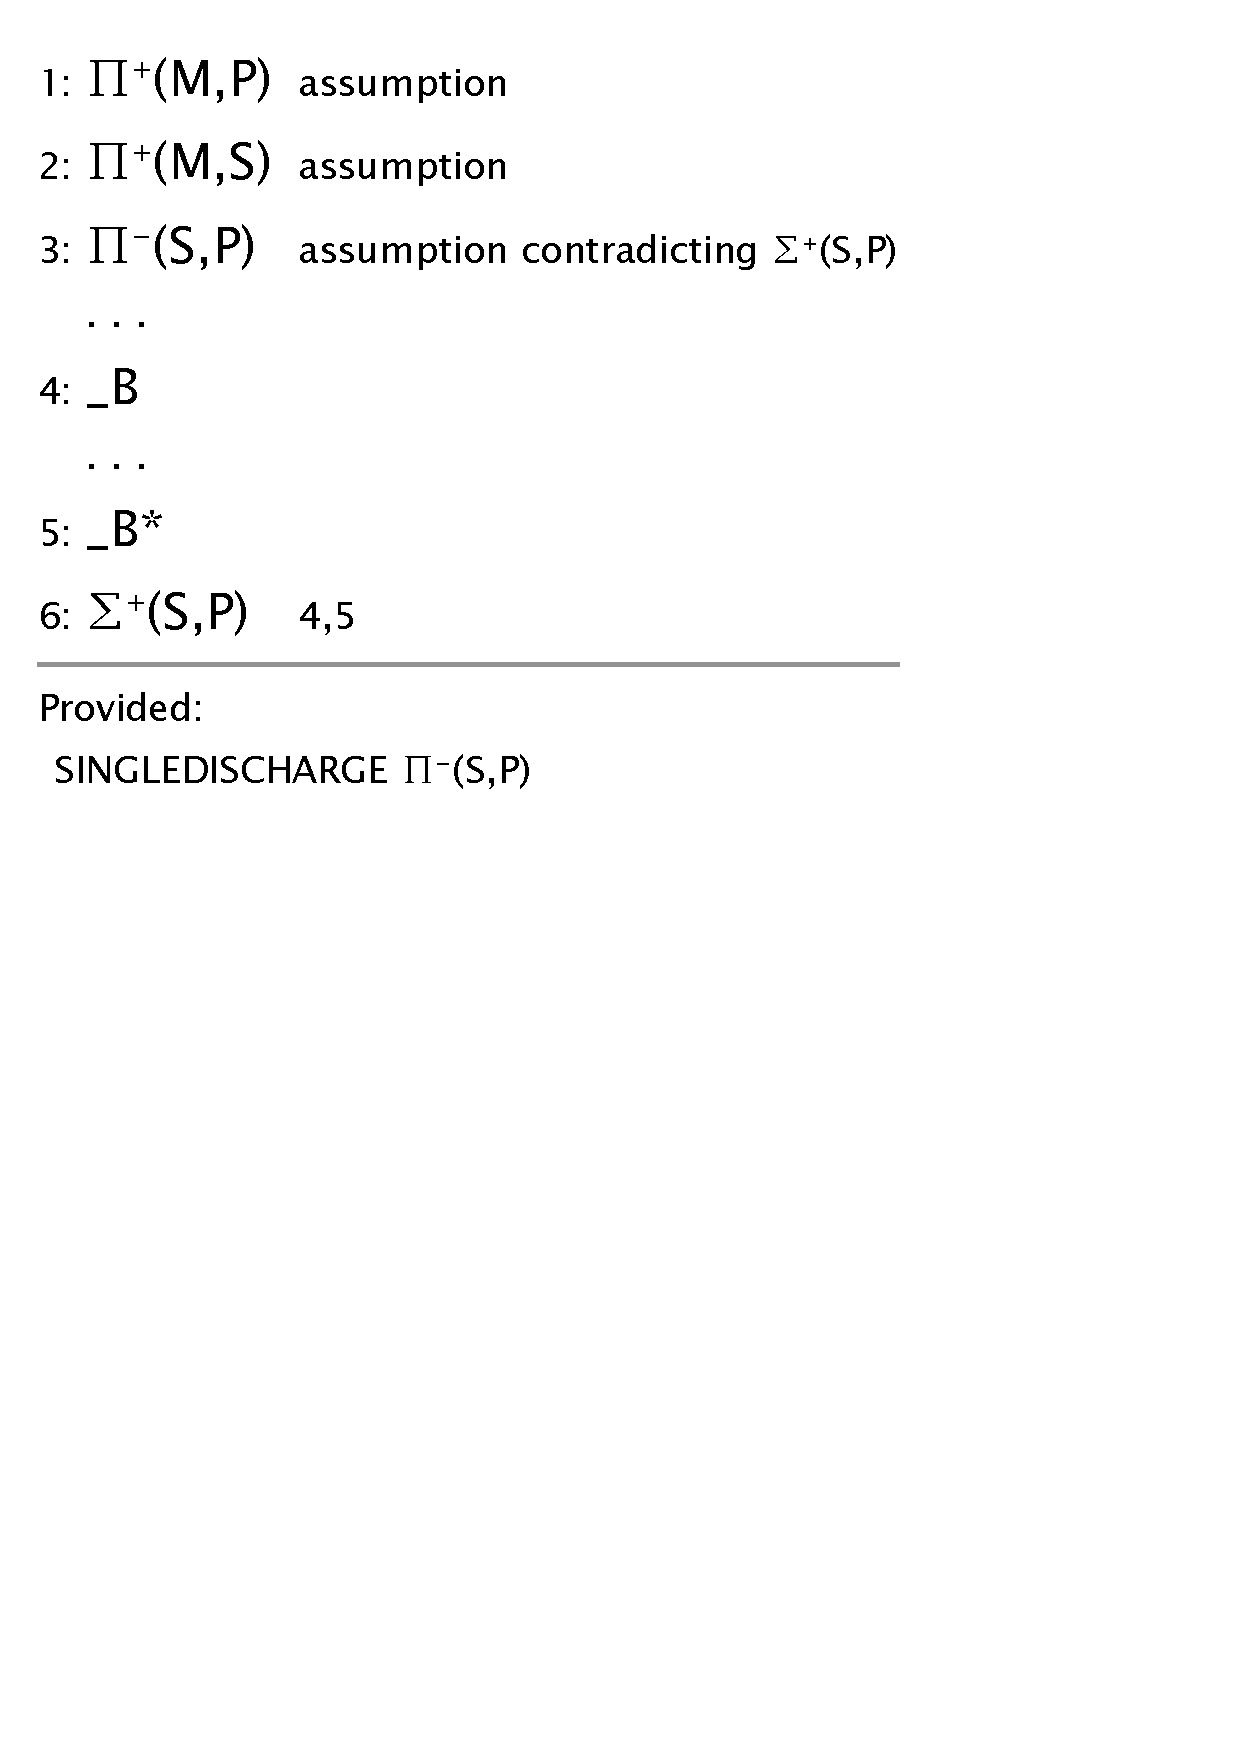
\includegraphics[scale=0.5]{pics/Aristotle/Darapti_0}
\end{quote}
If the proof develops so that we can determine \textj{\_B} on line 4 then the automatic application of a special rule will make the asterisk disappear:
\begin{japeish}
RULES contra ARE \\
\tab\tab\tab   FROM ∏⁺(S,P) INFER ∑⁻(S,P)*  \\
\tab AND FROM ∏⁻(S,P) INFER ∑⁺(S,P)*    \\  
\tab AND FROM ∑⁺(S,P) INFER ∏⁻(S,P)*  \\
\tab AND FROM ∑⁻(S,P) INFER ∏⁺(S,P)*  \\
END\\
\\
TACTIC "contra-tac" IS LAYOUT HIDEROOT contra\\
\\
AUTOMATCH "contra-tac"
\end{japeish}
\begin{figure}
\centering
\subfigure[first stage of proof]{\centering
\makebox[170pt]{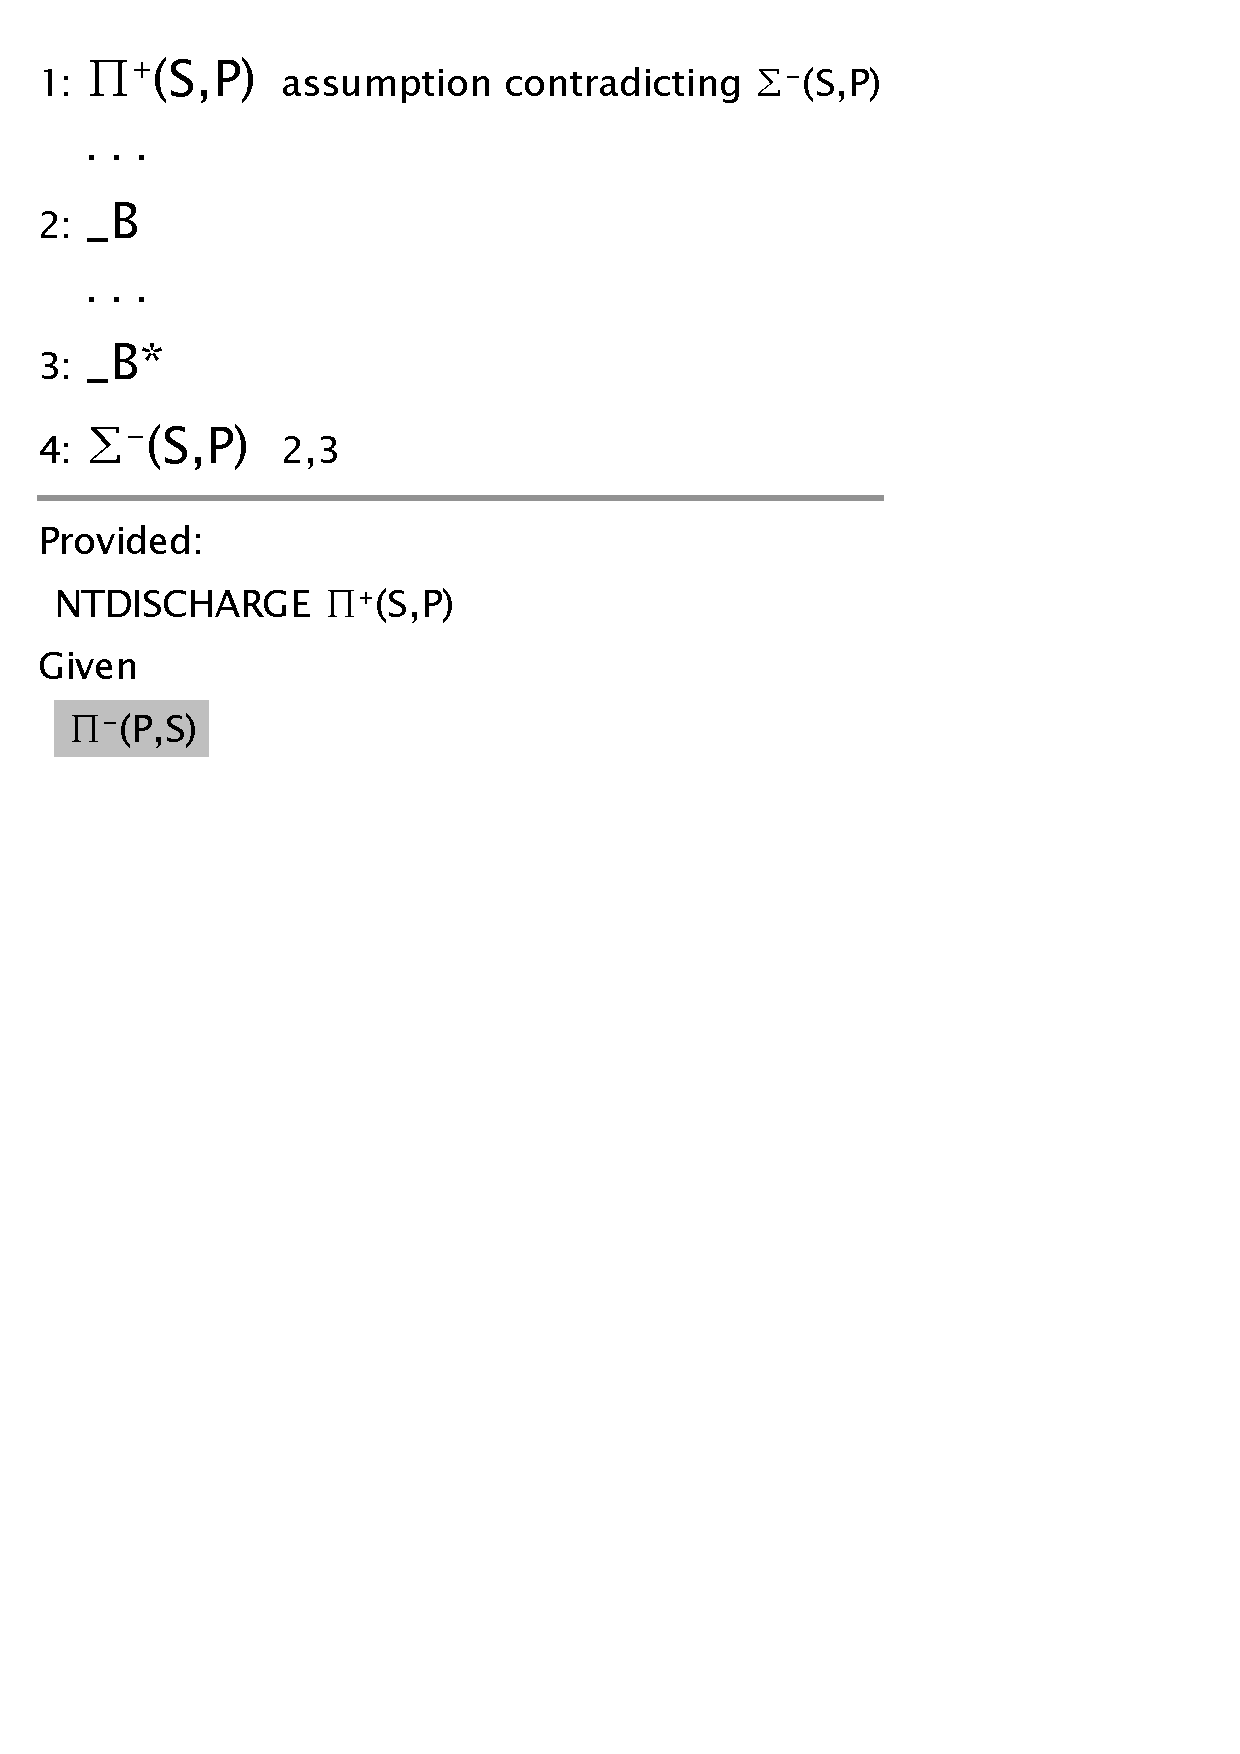
\includegraphics[scale=0.4]{pics/Aristotle/subaltern_0}}\label{fig:Aristotle:subaltern_0}}
\subfigure[after Given is applied to line 3]{\centering
\makebox[170pt]{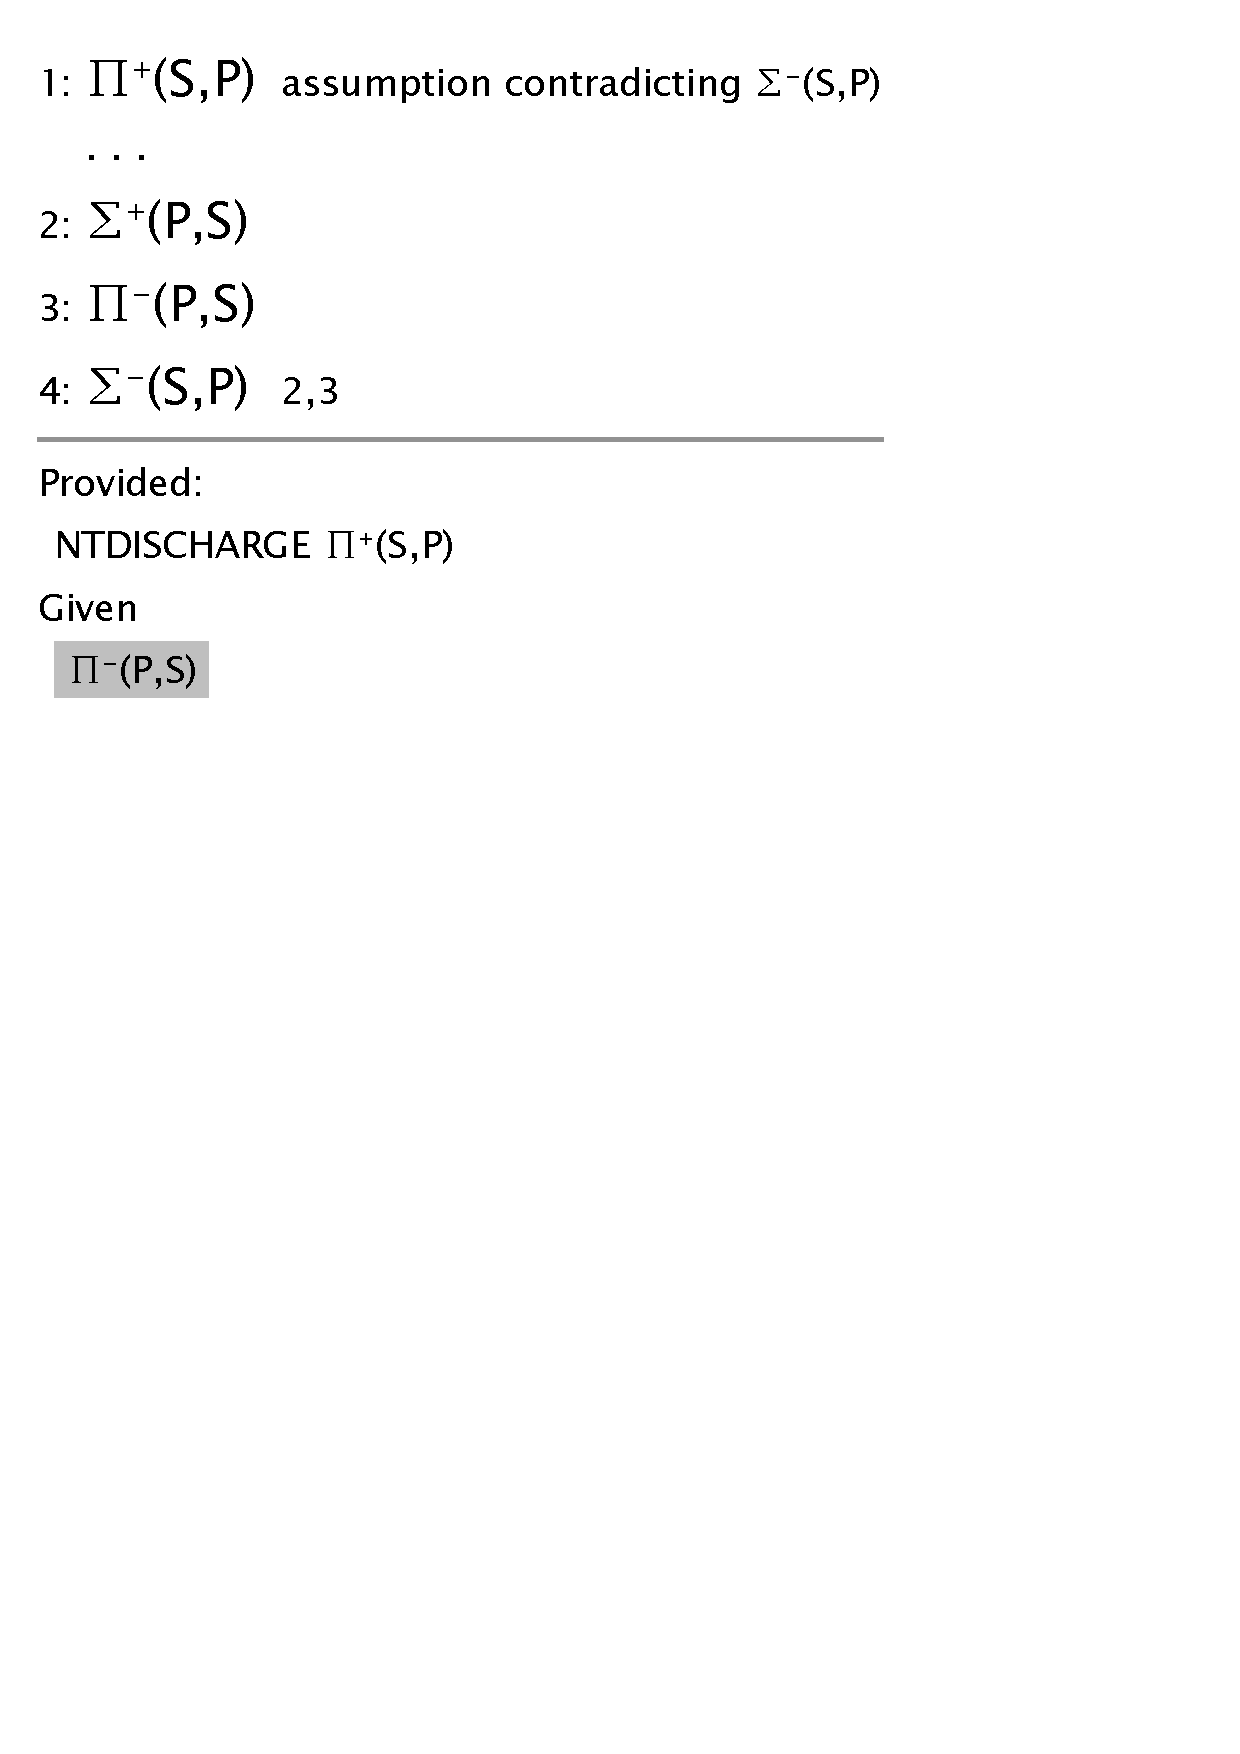
\includegraphics[scale=0.4]{pics/Aristotle/subaltern_1}}\label{fig:Aristotle:subaltern_1}}
\caption{Proving a derived rule}
\label{fig:Aristotle:subaltern_various}
\end{figure}
Indeed, that's most often what happens. But not always: sometimes we discover what \textj{\_B*} should be, and we want to use \textj{see}, or a Given formula, to determine it. Figure \ref{fig:Aristotle:subaltern_0}, for example, is the first stage of the proof of a derived subaltern rule. There is absolutely nothing that \textj{\_B*} on line 3 can be, other than the Given \textj{∏⁻(P,S)}. We don't want to have to calculate what \textj{\_B} must be: surely the encoding of the theory should do that. 

There's a rule \textj{dcontra}, a tactic \textj{remstar} that uses it, and a tactic \textj{dogiven} that uses \textj{remstar}; \textj{dogiven(0)} is the tactic that is applied by selecting the formula on line 2 and clicking \textj{∏⁻(P,S)} in the Given menu:
\begin{japeish}
INITIALISE givenMenuTactic dogiven\\
\\
TACTIC dogiven(i) IS SEQ remstar (GIVEN i) \\
\\
TACTIC remstar IS \\
\tab  WHEN (LETGOAL (\_A*) (LAYOUT HIDEROOT dcontra))\\
\tab\tab\tab\tab       SKIP\\
\\       
RULE dcontra IS FROM A INFER A**
\end{japeish}
\textj{remstar} either applies \textj{dcontra} or \textj{SKIP}. Applied to the goal \textj{\_B*}, the \textj{LETGOAL} guard succeeds, and it applies \textj{dcontra}; the rule unifies \textj{\_B*} with \textj{\_A1**} -- i.e. it unifies \textj{\_B} with \textj{\_A1*}, producing the antecedent goal \textj{\_A1}. Then \textj{GIVEN 0} unifies \textj{\_A1} with \textj{∏⁻(P,S)}. Since \textj{\_B} is now \textj{∏⁻(P,S)*}, \textj{contra-tac} tidies up, and we have the proof state in figure \ref{fig:Aristotle:subaltern_1}.

But there's a subtlety. Suppose we select \textj{\_B} on line 2 of figure \ref{fig:Aristotle:subaltern_0} and click \textj{∏⁻(P,S)} in the Given menu. That would apply \textj{dogiven 0}, which would apply \textj{remstar}. Should \textj{LETGOAL (\_A*)} succeed? Certainly \textj{\_B} and \textj{\_A*} unify, but only by changing the proof, replacing \textj{\_B} by \textj{\_A*} and \textj{\_B*} by \textj{\_A**}. That seems to me to be an error: asking whether a proof element has a particular shape should not alter that element. Applying a rule can change the tree, but asking a question should not. So \textj{LETGOAL (\_A*)} will fail on line 2, \textj{remstar} will do nothing, and \textj{GIVEN 0} will unify \textj{\_B} with \textj{∏⁻(P,S)}, as it should (though it's actually the wrong move to make at that point in the proof).

The rest of the encoding is fairly straightforward, though it makes a lot of use of \textj{CUTIN} and \textj{see}, to make the \textj{priorAntes} mechanism work.
